% Outline Project Specification Report

%The document is a report
\documentclass[12pt,a4paper]{article}

%define horizontal rule
\newcommand{\HRule}{\rule{\linewidth}{0.5mm}}

\usepackage{fullpage}

%use the listings package
\usepackage{listings}
%use the English language
\usepackage[english]{babel}
%use graphics
\usepackage{graphicx}
%use wrap figures
\usepackage{wrapfig}
%geometry stuffs
\usepackage{lscape}
%use natbib bibliography package
%\usepackage[numbers]{natbib}
%use harvard bibliography package
%\usepackage{harvard}	
%use captions
\usepackage{caption}
%use multi-row tables
\usepackage{multirow}
\usepackage{url}

\begin{document}

%use harvard citations
%\citationstyle{agsm}

%include the title page
\begin{titlepage}
 
\begin{center}

% Upper part of the page

\includegraphics[width=0.20\textwidth]{../cover_logo.png}\\[1cm]


\textsc{\LARGE Aberystwyth University}\\[0.5cm]
\textsc{\LARGE Final Report}\\[0.5cm]



 
% Title
\HRule \\[0.4cm]
{ \huge \bfseries Partridge: An Intelligent Literature Analysis and
Recommendation Suite.}\\[0.4cm]

\HRule \\[1.5cm]

 % Author and student ID
\begin{minipage}{0.4\textwidth}
\begin{flushleft} \large
\emph{Author:}\\
\textsc{James Ravenscroft}\\
jrr9@aber.ac.uk\\
090407039\\
\end{flushleft}
\end{minipage}
\begin{minipage}{0.4\textwidth}
\begin{flushright} \large
\emph{Supervisors} \\
Amanda Clare (afc)\\
Maria Liakata (mal)

\end{flushright}
\end{minipage}


\vfill

\textsc{Submitted in partial fulfilment of requirements for a Batchelor of
Science Degree at Aberystwyth University}



\vfill
 
% Bottom of the page
\textsc{\large Word Count: 0}\\
\textsc{\large Status: Draft}\\
\textsc{\large Revision: \Revision{} }\\
{\large \today}
 
\end{center}

\frontmatter
 
\end{titlepage}



%some definitions for paragraph layout stuff
\setlength{\parindent}{0pt}
\setlength{\parskip}{1.5ex plus 0.5ex minus 0.2ex}

\tableofcontents

\pagebreak

\section{Project Summary}

\subsection{Introduction}
Partridge is a web-based tool designed to assist in information processing and knowledge
acquisition in the domain of scientific research.

Since the advent of the 'Digital Age' and the ability of computers to copy and
reproduce information for a negligible cost, the amount of information
available to researchers has been increasing drastically.  A 2009 study by B-C
Bj\"{o}rk suggests that approximately 1.4 Million papers were published in the
year 2006 alone\cite{bjork2009}. Moreover, the growing popularity of Open Access
publishing (making papers available for free online\cite{Suber2012}) across
most scientific disciplines is providing researchers with an even larger volume
of information to be processed. As the amount of available information grows,
relevant material becomes increasingly difficult to find and the need for an
automated information retrieval tool is ever more apparent.

Partridge aims to autonomously process as many scientific papers as possible to
facilitate researchers who would otherwise be required to manually read each
paper themselves. This should reduce the amount of information that the user is
required to process themselves, thereby speeding up the research process.
Partridge will achieve this through the use of several existing techniques in
the field of Natural Language Processing which are discussed below.

From the point of view of it's users, Partridge will assist researchers in two
ways. The system will provide filtering of papers based upon their
specific domain (i.e. is the paper primarily concerned with methodology within
an experiment in chemistry or is it about Ethics in Psychological studies?) and
their result, whether the paper yielded positive, negative or inconclusive
evidence for a hypothesis. Depending upon the time constraints of the
project, it is hoped that Partridge will also offer a user 'profiling' system
that provides recommendations for researchers based on their reading history.
This feature should help users find relevant papers more quickly or find research that
they may have otherwise overlooked.

To facilitate the above behaviour, Partridge will make use of Natural
Language Processing (NLP) techniques. NLP enables the automated extraction of
meaningful information from texts written in human languages such as English or
French. 

\section{Current Progress}

\subsection{Prior Art}

Within the field of scientific research and on the internet in general, there
are already several systems for assisting users in retrieving useful and
relevant information.

There are many existing search engines for finding information on the internet
in general. Most people have heard of Google (\url{http://wwww.google.com}),
and Yahoo (\url{http://www.yahoo.co.uk}), Bing (\url{http://www.bing.com}) and Ask
(\url{http://www.ask.com}). There are many more similar systems available for free
general use across the internet. They all present very similar user interfaces in
which users are asked to supply keywords that might be linked to relevant documents 
and the search engine returns a list of Uniform Resource Locators (URLs) that they 
consider to match the user's query. 

These search engines are often helpful in locating other pages within the World Wide
Web. Unfortunately, the results they provide are usually too general to find
scientific papers and journals. Search engines also index a huge proportion of
irrelevant information compared to useful information\cite{Berghel1997}, and as
a result, even relatively specific queries such as effects of gravity on rockets" yield
millions of results (as shown in Figure \ref{fig:rocket_results}). 

\begin{figure}[!ht]
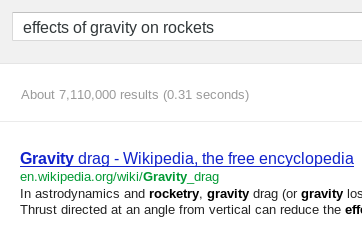
\includegraphics[width=0.80\textwidth]{images/space_rocket_query.png}
\caption{{Google showing over 7M results for ``effects of gravity on rockets"}}
\label{fig:rocket_results}
\end{figure}

There are also a number of search and indexing systems available for locating
scientific papers by keyword or through the use of metadata to make
recommendations. One of the most publicised paper search system is Google
Scholar. This is an adaptation of Google's general search algorithm to
specifically handle scientific papers. 

\section{Planning}

\pagebreak
\bibliographystyle{IEEEannot}
\bibliography{report}

\end{document}
